% ----------------------------------------------------------
\chapter{Resultados}
% ----------------------------------------------------------
\section{Hospedagem e Publicação}

O Balmy.jl foi publicado utilizando o GitHub Pages, uma ferramenta gratuita para serviços fornecidos por APIs. Ele hospeda sites estáticos criados a partir de repositórios Git, um sistema de controle de versões distribuído, usado principalmente no desenvolvimento de \textit{software}, pois salva todo o histórico de edições contido no processo de construção de um programa computacional. 

\section{Interface gráfica}

A interface gráfica construída é devidamente mostrada na \autoref{gui-pronta}. Os elementos interativos foram implementados para fazer com que o \textit{software} em questão fosse o mais amigável possível ao usuário, isto é, extremamente intuitivo e fácil de usar, podendo ser acessado através do navegador e, assim, utilizado nas salas de aula da graduação.

\begin{figure}[htb]
	\caption{\label{gui-pronta} Aqui é mostrada a interface gráfica produzida. Os círculos sinalizam as funções associadas às áreas da GUI (\textit{Graphical User Interface})}
	\begin{center}
		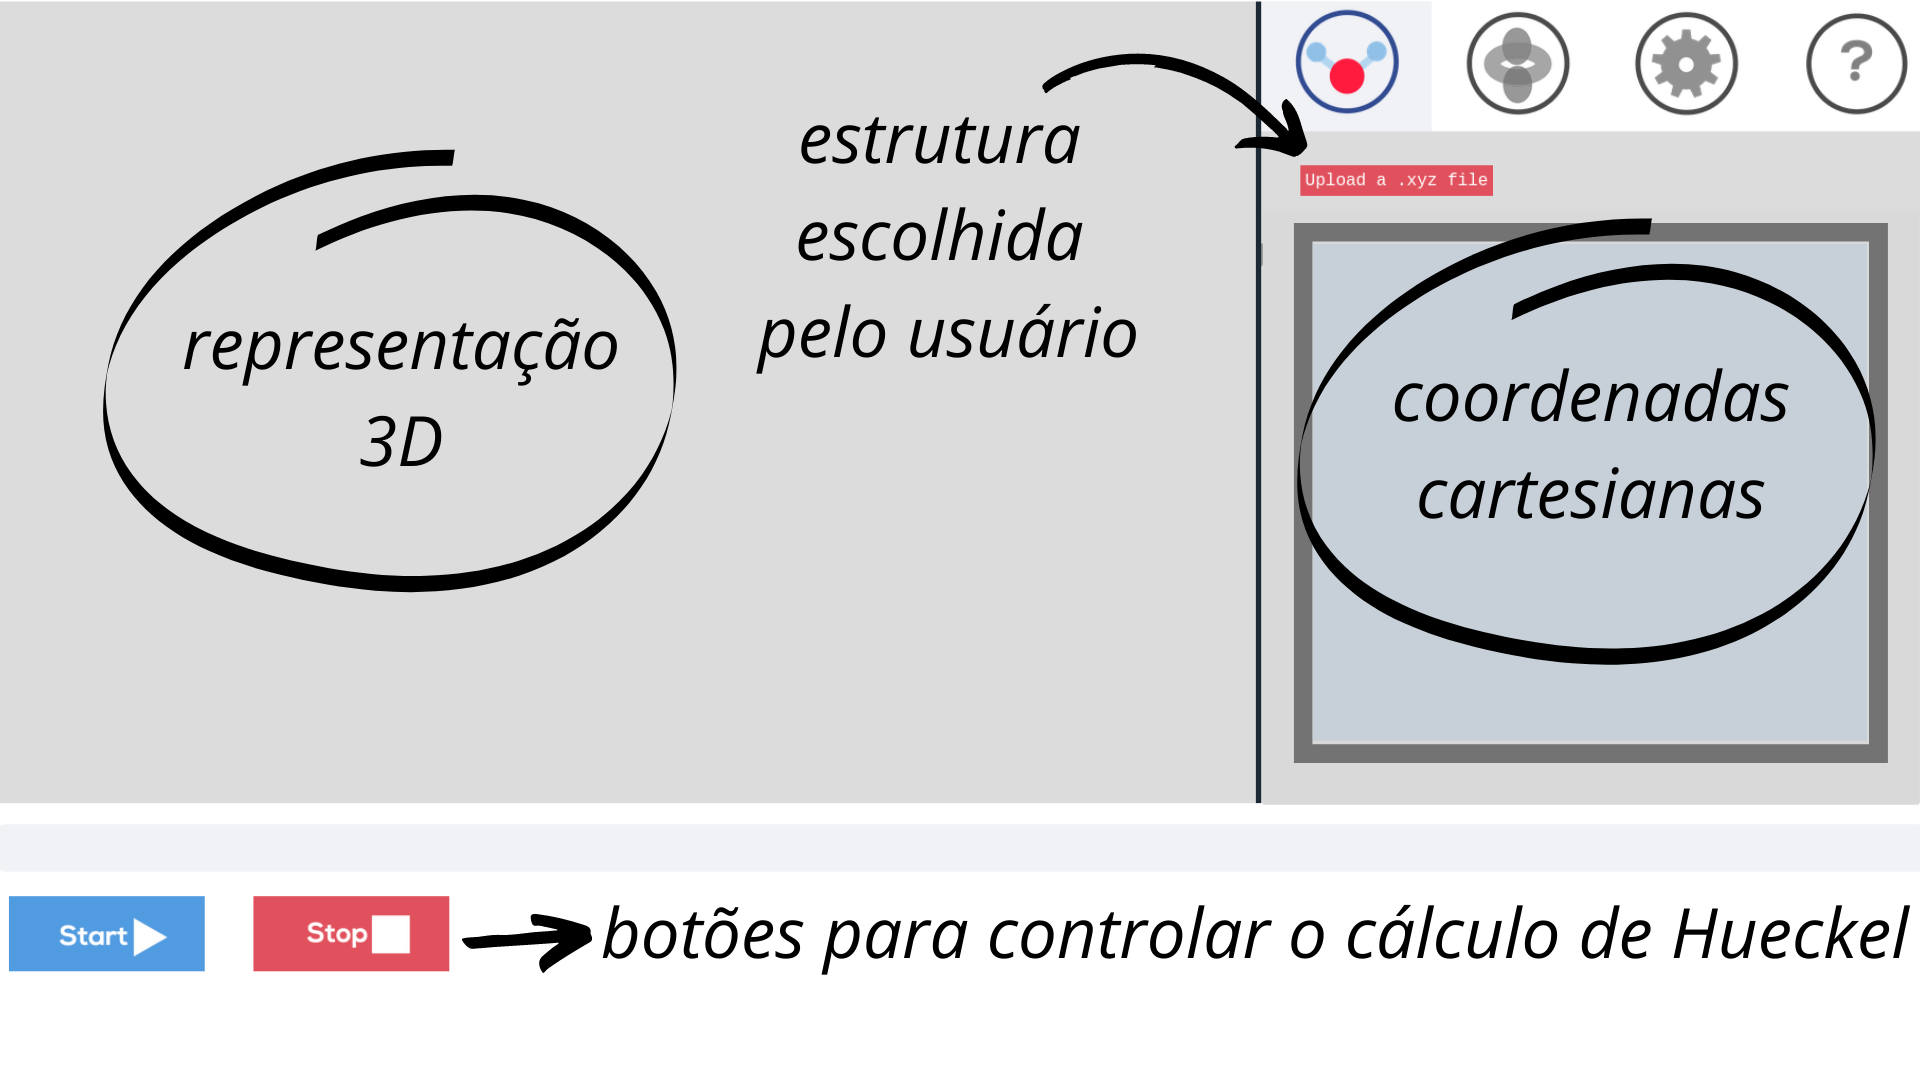
\includegraphics[width=1.0\textwidth]{images/GUI-EXAMPLE.png}
	\end{center}
	\fonte{Autor(a)}
\end{figure}

O fluxo de trabalho básico de funcionamento do WeBalmy.jl também é ilustrado pelo esquema da \autoref{workflow}, onde é possível notar que o usuário insere, como entrada, o arquivo contendo as coordenadas cartesianas do sistema químico que deseja estudar. A partir de tais informações, a estrutura é processada é representada tridimensionalmente e as energias dos seus orbitais moleculares são calculados pelo cálculo de Hueckel estendido, através do qual é possível fazer análises do caráter aromático presente na estrutura.

\begin{figure}[htb]
	\caption{\label{workflow} Fluxo de trabalho do \textit{software} produzido.}
	\begin{center}
		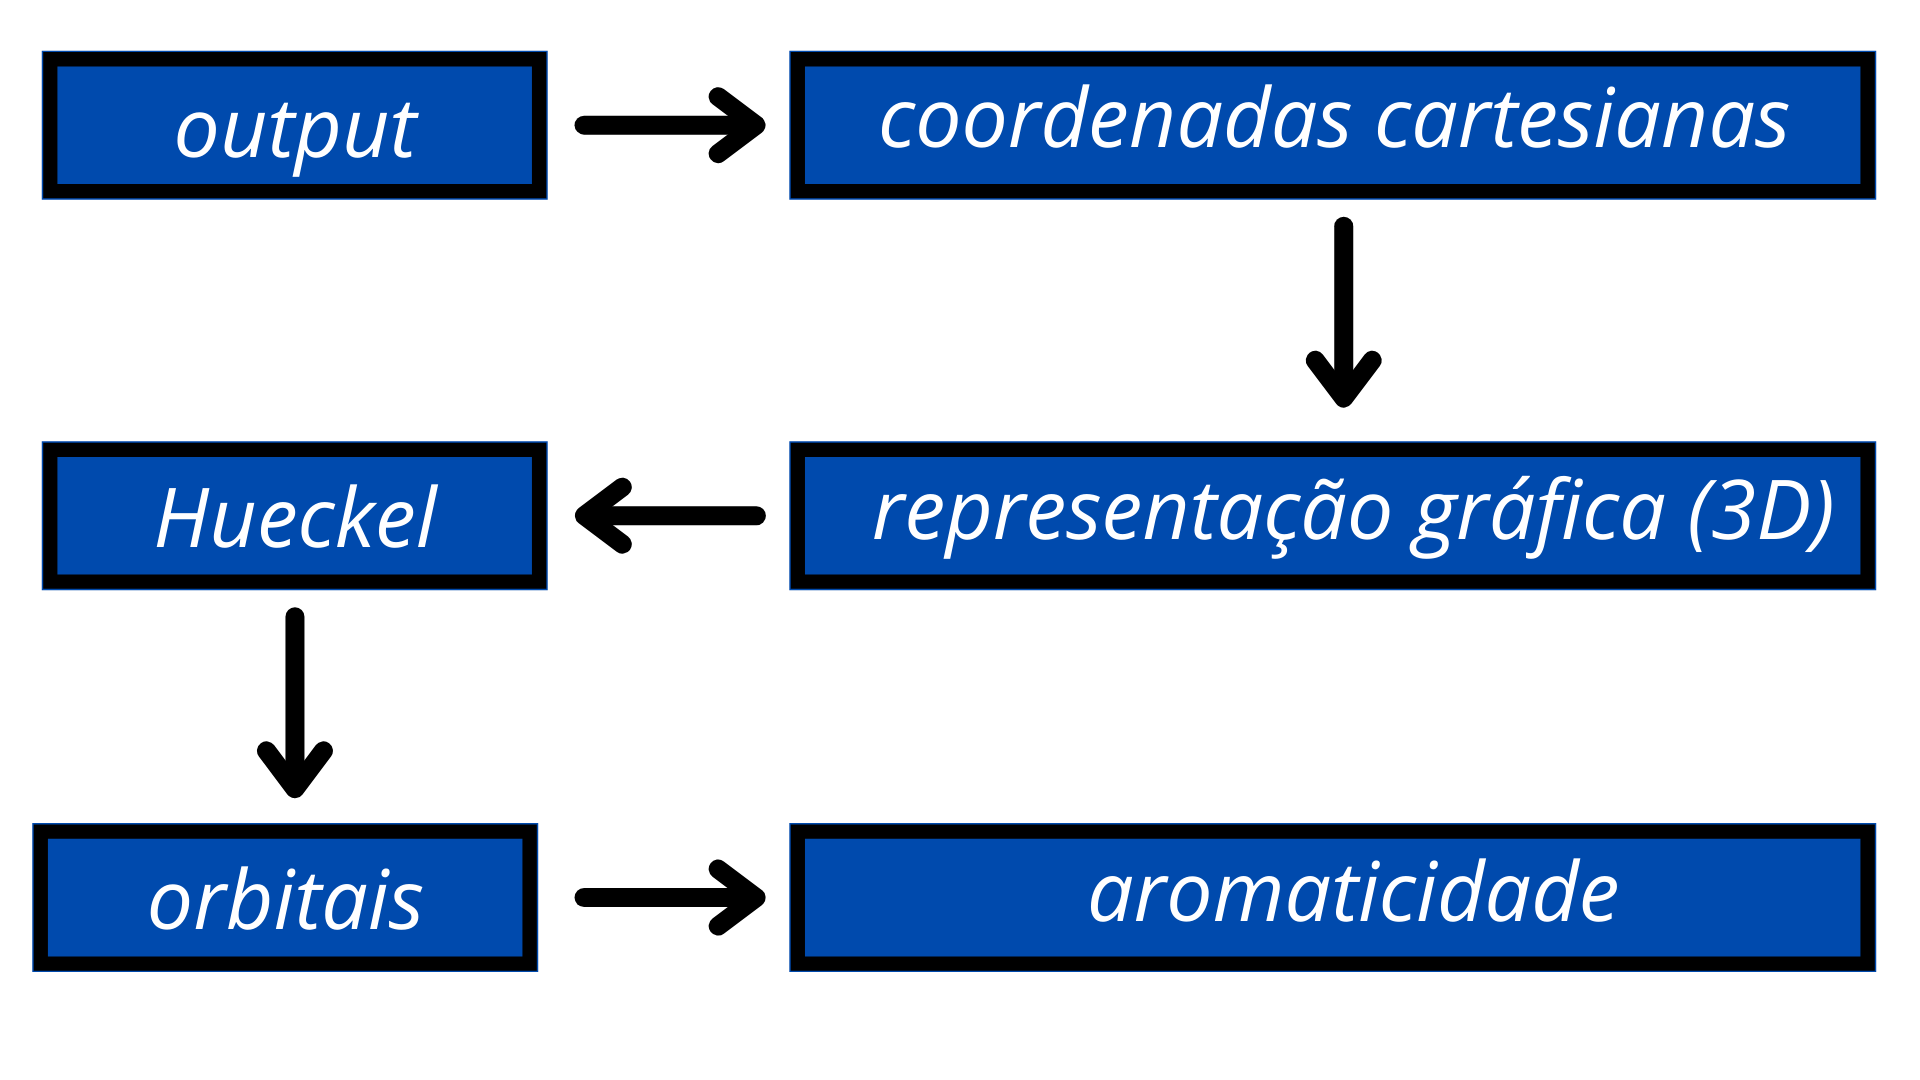
\includegraphics[width=0.65\textwidth]{images/workflow.png}
	\end{center}
	\fonte{Autor(a)}
\end{figure}

\section{Representação tridimensional}

Para representar os modelos tridimensionais utilizando o Three.js, é utilizado o modelo de Blinn-Phong, capaz de simular superfícies brilhantes com holofotes especulares. O sombreamento é calculado \textit{per pixel} de acordo com o modelo de Phong. Desse modo, apesar de custar um pouco mais de tempo para renderizar, ele atinge uma acurácia maior do que outros modelos disponíveis (o de Lambert, por exemplo).

No modelo primeiramente proposto por Phong, é calculado continuamente o produto escalar $R \cdot V$ entre um observador $V$ e o feixe de uma fonte de luz ($L$) refletida ($R$) sobre uma superfície. No ajuste proposto por Blinn, no entanto, calcula-se um vetor a meio caminho entre o espectador e os vetores de fonte luminosa, podendo substituir $R \cdot V$ por $N \cdot H$, onde $N$ é o vetor normal à superfície.

\begin{figure}[htb]
\begin{equation}
    \label{eq:R1}
    H = \frac{L + \highlight{blue}{V} }{||L + \tikzmarknode{value}{\highlight{blue}{V}}||}
\end{equation}
\begin{tikzpicture}[overlay,remember picture,>=stealth,nodes={align=left,inner ysep=1pt},<-]
    \path (value.south) ++ (-1,-1.5em) node[anchor=north east,color=blue!67] (scalep){\textit{$V = P_H (-L)$}};
    \draw [color=blue!87](value.south) |- ([xshift=-1.65em,color=blue]scalep.north west);
\end{tikzpicture}
\vspace{2\baselineskip}
\end{figure}

Na \autoref{eq:R1}, $P_H$ é a matriz de Householder que reflete um ponto no hiperplano que contém a origem e tem um vetor normal $H$. Este produto escalar é o cosseno de um ângulo que é metade do ângulo representado pelo produto escalar de Phong (se $V$, $L$, $N$ e $R$ estiverem todos no mesmo plano). Esta relação entre os ângulos sofre desvios discretos quando os vetores não se encontram no mesmo plano, especialmente em relação aos ângulos pequenos.

Ainda sobre os ajustes de Blinn ao modelo de Phong, consideremos que o ângulo entre o vetor a meio caminho $(N \cdot H)$ e a superfície normal é provavelmente menor do que o ângulo entre $R$ e $V$ usado no modelo original (a menos que a superfície seja vista de um ângulo muito íngreme para o qual é provável que seja maior), e já que Phong está usando $(R \cdot V)^\alpha$, um expoente (chamado de constante de brilho) pode ser definido como $\alpha' > \alpha$, tal que $(N \cdot H)^{\alpha'}$ está mais próxima da expressão original de Phong.

\begin{figure}[htb]
\caption{\label{fig:representations} Exemplo da aplicação do modelo de Blinn-Phong na molécula de benzenos a partir da alteração dos coeficientes $\alpha'$ para os átomos (representados por esferas). Da direita para a esquerda, os valores atribuídos foram: 0, 10, 50, 100, 1000; respectivamente.}
	\begin{center}
		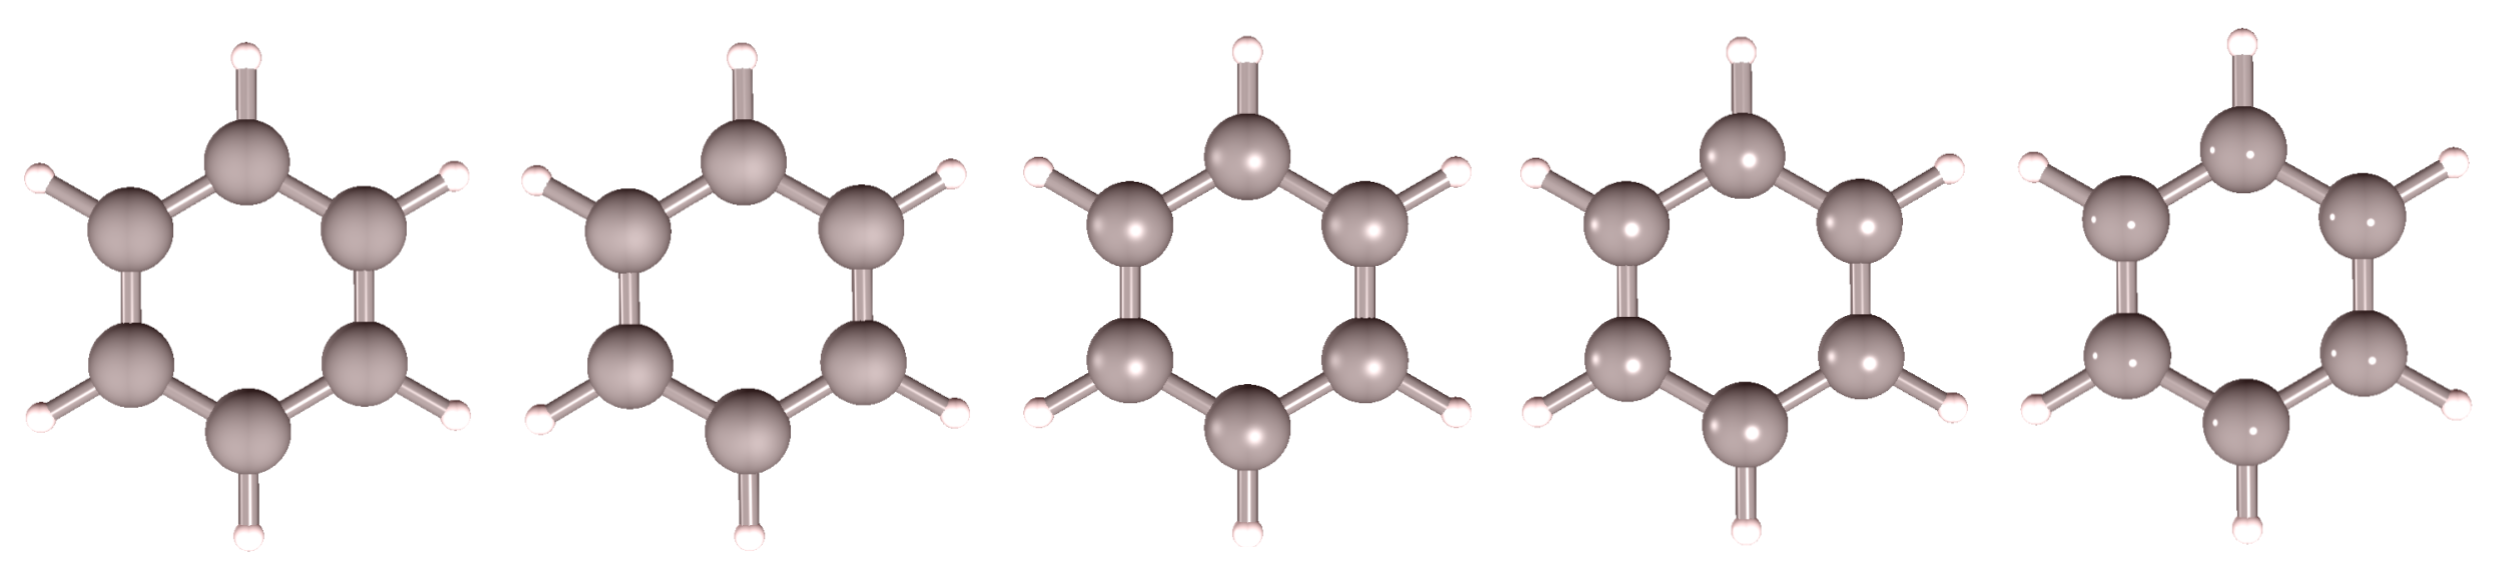
\includegraphics[width=1.0\textwidth]{images/shininess(1).png}
	\end{center}
	\fonte{Autor(a)}
\end{figure}

Variando, portanto, o valor de $\alpha'$, é possível notar que, na \autoref{fig:representations}, quanto maior for seu valor, menor será o holofote especular, representado pelos pontos luminosos nas estruturas moleculares.

\section{Hidrocarbonetos aromáticos}

Analisando os dados da \autoref{tab:energies}, concluímos que a ordem das estabilidades dos compostos está de acordo com aqueles apresentados por Hoffmann \autocite{Hoffmann1963}, e com os dados experimentais publicados por Heilbronner \autocite{ginsburg1959}. Por exemplo, o naftaleno mostra-se 32.3 kcal/mol mais estável do que o azuleno, o que é um ótimo resultado se comparado com o valor de referência (32.6 kcal/mol)\autocite{ginsburg1959}. O fulveno, por sua vez, é computado como sendo 25.6 kcal/mol menos estável do que o benzeno, em relação ao valor de 27 kcal/mol tomado como modelo\autocite{CHENG1956}. O antraceno, por sua vez, é 4.2 kcal/mol mais estável do que o fenantreno, enquanto o último isômero é, na verdade, 6.9 kcal/mol mais estável \autocite{Hoffmann1963}, o que provém do fato de que há repulsão estérica entre os hidrogênios do fenantreno.

\begin{table}[htb]
	\centering
	\caption{\label{tab:energies} Energias dos elétrons $\pi$ nos compostos aromáticos.}	
	\begin{tabular}{lrr}
		\toprule
		\textbf{Molécula} & $E_\pi / (eV)$ & $E_\pi / (kcal/mol)$
		\\ 
		\midrule
        Etileno & -26.336 & -609.628 \\
        Butadieno & -52.964 & -1221.38 \\
        Benzeno & -80.208 & -1849.64 \\
        Fulveno & -78.928 & -1820.12 \\
        Naftaleno & -133.676 & -3082.64 \\
        Azuleno & -132.934 & -3065.53 \\
        Fenantreno & -187.286 & -4318.92 \\
        Antraceno & -187.020 & -4312.78 \\
    \bottomrule
	\end{tabular}
	\fonte{Autor(a).}
\end{table}

\section{Diagramas de orbitais moleculares}

Seguindo o grafo mostrado na \autoref{fig:M2} e enumerado na \autoref{fig:graphEnumerated}, é possível construir uma matriz de adjacência de dimensão $n \times n$, onde $n$ é o número de átomos, excluindo-se os hidrogênios. No caso do benzeno, a ordem da matriz em questão é 6.

\begin{figure}[htb]
\vspace{0.8\baselineskip}
\begin{equation}
\label{eq:adjmatrix}
\begin{bmatrix}
    0 & 1 & 0 & 0 & 0 & 1 \\
    1 & 0 & 1 & 0 & 0 & 0 \\
    0 & 1 & 0 & 1 & 0 & 0 \\
    0 & 0 & 1 & 0 & 1 & 0 \\
    0 & 0 & 0 & 1 & 0 & 1 \\
    1 & 0 & 0 & 0 & 1 & 0
\end{bmatrix}
\end{equation}
\end{figure}

\noindent Consideremos $a_{ij}$ o elemento geral associado à matriz da \autoref{eq:5}, sendo igual a uma unidade quando os carbonos $i$ e $j$ estão ligados. Analogamente, na teoria de Hueckel e de Hueckel estendido, a matriz do determinante secular (\autoref{eq:secularmatrix}) é aquela cujos autovalores determinam as energias dos orbitais moleculares.

\begin{figure}[htb]
\vspace{0.8\baselineskip}
\begin{equation}
\label{eq:secularmatrix}
\begin{bmatrix}
    \alpha - E & \beta & 0 & 0 & 0 & \beta \\
    \beta & \alpha - E & \beta & 0 & 0 & 0 \\
    0 & \beta & \alpha - E & \beta & 0 & 0 \\
    0 & 0 & \beta & \alpha - E & \beta & 0 \\
    0 & 0 & 0 & \beta & \alpha - E & \beta \\
    \beta & 0 & 0 & 0 & \beta & \alpha - E \\
\end{bmatrix}
\end{equation}
\end{figure}

No caso do benzeno, ao resolver o determinante secular da matriz anterior (através do procedimento mostrado no \autoref{ap:HMO} e no \autoref{ap:EHMO}), obtemos a equação

\begin{figure}[htb]
\begin{equation}
    \label{eq:R3}
    \tikzmarknode{variable}{\highlight{blue}{$x$}}^6 - 6\highlight{blue}{$x$}^4 + 9\highlight{blue}{$x$}^2 = 0
\end{equation}
\begin{tikzpicture}[overlay,remember picture,>=stealth,nodes={align=left,inner ysep=1pt},<-]
    \path (variable.south) ++ (1,-1.5em) node[anchor=north west,color=blue!67] (scalep){\textit{$x = \displaystyle \frac{\alpha - E}{\beta}$}};
    \draw [color=blue!87](variable.south) |- ([xshift=1.65em,color=blue]scalep.north east);
\end{tikzpicture}
\vspace{2\baselineskip}
\end{figure}

\begin{figure}[htb]
\vspace{2\baselineskip}
\begin{equation}
    \label{eq:orb_mols}
\begin{split}
    \tikzmarknode{e1}{\highlight{blue}{$E_1$}} = \alpha +  2 \beta \\[0.3cm]
    \tikzmarknode{e2}{\highlight{red}{$E_2 = E_3$}} = \alpha + \beta \\
    \tikzmarknode{e3}{\highlight{red}{$E_4 = E_5$}} = \alpha - \beta \\[0.3cm]
    \tikzmarknode{e6}{\highlight{blue}{$E_6$}} = \alpha - 2\beta
\end{split}
\end{equation}
\begin{tikzpicture}[overlay,remember picture,>=stealth,nodes={align=left,inner ysep=1pt},<-]
    \path (e1.north) ++ (1,1.5em) node[anchor=south west,color=blue!67] (scalep){\textit{HOMO-1}};
    \draw [color=blue!87](e1.north) |- ([xshift=1.65em,color=blue]scalep.south east);

    \path (e2.north) ++ (-0.60,0.6em) node[anchor=south east,color=red!67] (scalep){\textit{HOMO (orbitais degenerados)}};
    \draw [color=red!87](e2.north) |- ([xshift=-1.65em,color=red]scalep.south west);
    
    \path (e3.south) ++ (-0.60,-0.6em) node[anchor=north east,color=red!67] (scalep){\textit{LUMO (orbitais degenerados)}};
    \draw [color=red!87](e3.south) |- ([xshift=-1.65em,color=red]scalep.north west);
    
    \path (e6.south) ++ (1,-1.5em) node[anchor=north west,color=blue!67] (scalep){\textit{LUMO+1}};
    \draw [color=blue!87](e6.south) |- ([xshift=1.65em,color=blue]scalep.north east);
\end{tikzpicture}
\end{figure}

Resolvendo o polinômio da \autoref{eq:R3}, conseguimos suas raízes ($x = \pm 1, \pm 1, \pm 2$) e, portanto, as energias para seis orbitais moleculares do benzeno (HOMO-1, HOMO, LUMO, LUMO+1). Combinando as raízes com os parâmetros $\alpha$ e $\beta$, nós temos a \autoref{eq:orb_mols} (\autoref{fig:MOs}).

\begin{figure}[htb]
\caption{\label{fig:MOs} Diagrama de energia dos orbitais moleculares do benzeno.}
	\begin{center}
		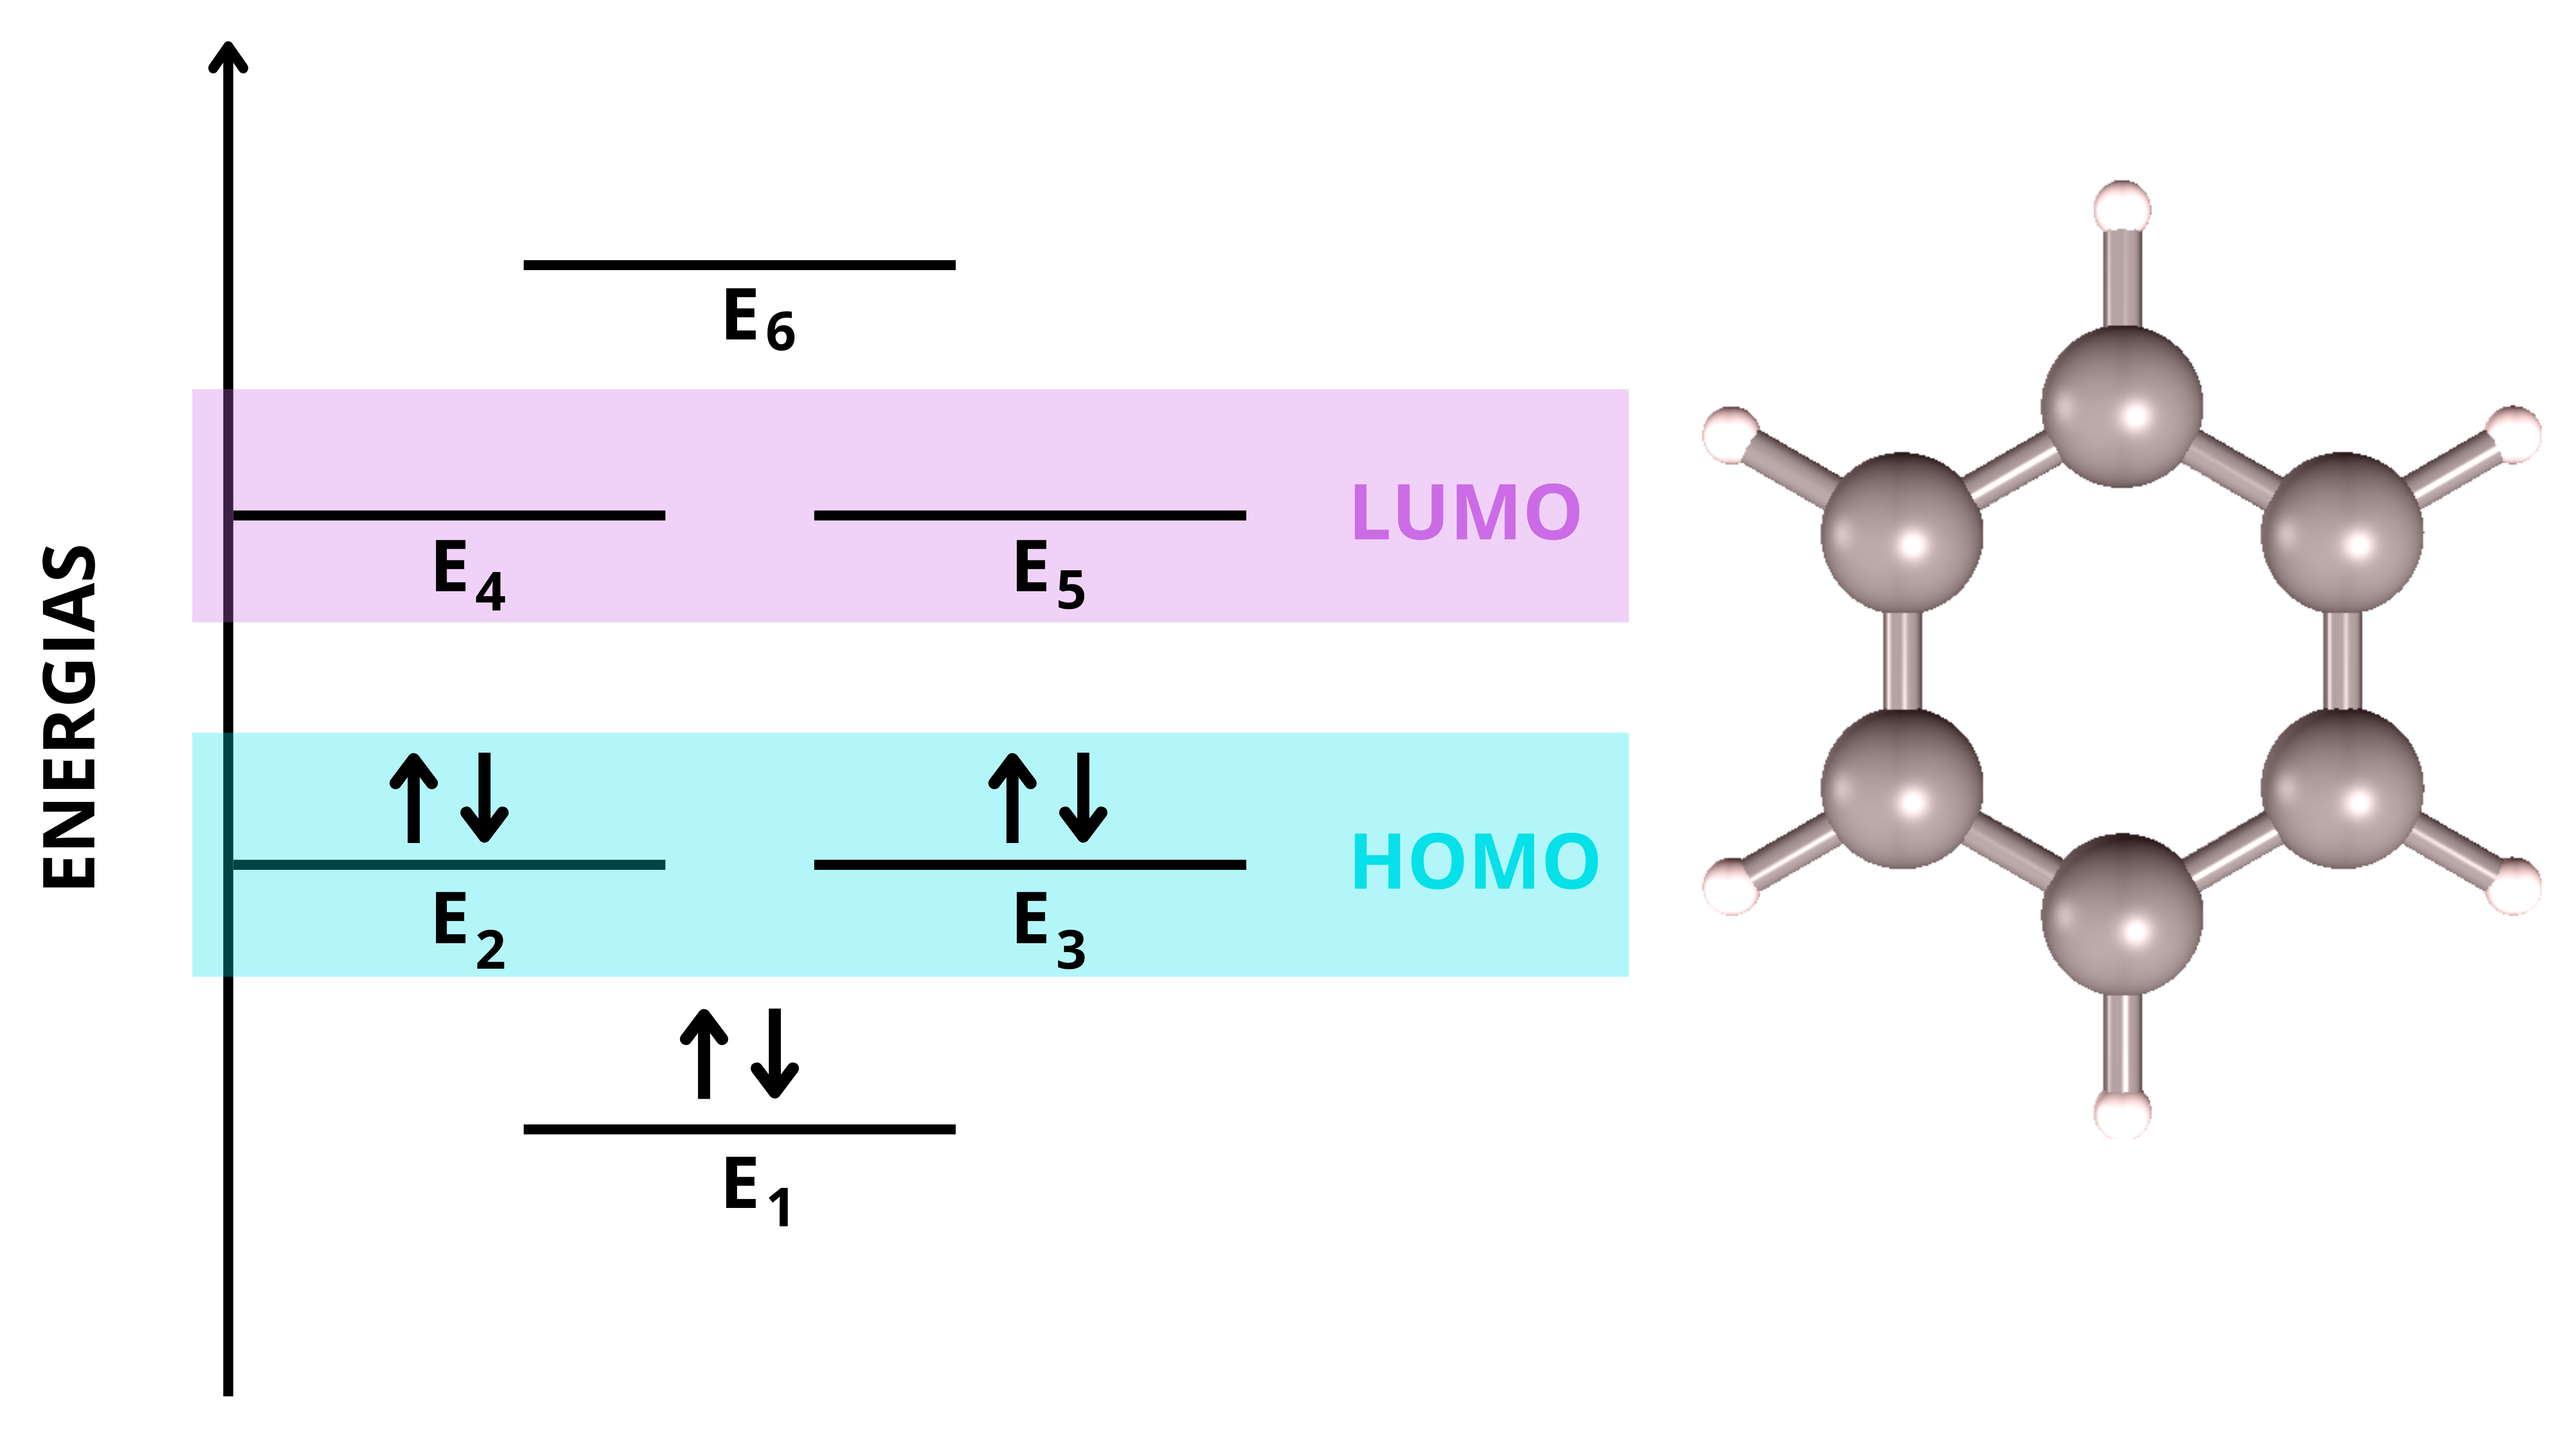
\includegraphics[width=0.75\textwidth]{images/MOs.png}
	\end{center}
	\fonte{Autor(a)}
\end{figure}

Os autovalores repetidos vão gerar orbitais degenerados, isto é, aqueles que estão no mesmo nível energético, como é possível notar no diagrama e nos valores de energia obtidos. Esses mesmos valores podem ser obtidos se calcularmos os autovalores da matriz de adjacência. Desse modo, comprovamos que, ao solucionar o determinante e os autovalores da matriz secular, é possível obter os valores de energia e as populações associadas a cada orbital molecular da molécula de interesse.

\begin{table}[htb]
	\centering
	\caption{\label{qua:Quadro_1} Energias dos orbitais de fronteira de alguns hidrocarbonetos aromáticos.}	
	\begin{tabular}{lrrr}
		\toprule
		\textbf{Molécula} & \textbf{HOMO/(eV)} & \textbf{LUMO/(eV)} & \textbf{Gap/(eV)}
		\\ 
		\midrule
        benzeno & -12.797 & -8.345 & 4.452 \\
        naftaleno & -12.073 & -9.338 & 2.635 \\
        antraceno & -11.642 & -9.839 & 1.803 \\
        fenantreno & -12.023 & -9.310 & 2.713 \\
        azuleno & -11.730 & -9.872 & 1.858 \\
        pentaleno & -11.492 & -10.809 & 0.683 \\
        fulveno & -11.991 & -10.338 & 1.653 \\
        bifenileno & -11.555 & -9.553 & 2.002 \\
        tolueno & -12.502 & -8.348 & 4.154 \\
    \bottomrule
	\end{tabular}
	\fonte{Autor(a).}
\end{table}

Como o enfoque desse trabalho é a análise de compostos aromáticos, analisaremos de maneira mais aprofundada o exemplo do benzeno, cujas coordenadas estão mostradas na \autoref{tab:coords}. Os comprimentos de ligação obtidos para \ce{C-C} são $1.40 \AA$ e, para \ce{C-H}, são $1.10 \AA$.

\begin{table}[htb]
	\centering
	\caption{\label{tab:coords} Coordenadas atômicas do benzeno.}	
	\begin{tabular}{crrr}
		\toprule
		\textbf{Átomo (posição)} & $x$ & $y$ & $z$
		\\ 
		\midrule
        C(1) &  1.40 &  0.00 & 0.00 \\ 
        C(2) & -1.40 &  0.00 & 0.00 \\
        C(3) &  0.70 &  1.21 & 0.00 \\
        C(4) &  0.70 & -1.21 & 0.00 \\
        C(5) & -0.70 & -1.21 & 0.00 \\
        C(6) & -0.70 &  1.21 & 0.00 \\
        H(1) &  2.50 &  0.00 & 0.00 \\
        H(2) & -2.50 &  0.00 & 0.00 \\
        H(3) &  1.25 &  2.16 & 0.00 \\
        H(4) &  1.25 & -2.16 & 0.00 \\
        H(5) & -1.25 & -2.16 & 0.00 \\
        H(6) & -1.25 &  2.16 & 0.00 \\
    \bottomrule
	\end{tabular}
	\fonte{Autor(a).}
\end{table}

\section{Influência de K}


\section{Índices geométricos}